\section{Resultados e discussões}
\subsection{Termoscópio}

Ao segurar o bulbo inferior de termoscópio, foi possível observar o nível da água subir pelo tubo. Similarmente, ao expor o termoscópio ao vento do ar condicionado da sala, foi possível observar o nível da água descer. Segurar o bulbo superior não causou modificação observável no termoscópio. 

A experiência é explicada pela variação de temperatura. Como o bulbo é de um vidro extremamente fino, ao segurar, a temperatura da mão e a temperatura do ar e da água no bulbo começam a entrar em equilíbrio. A mão, estando mais quente, transfere energia cinética para as moléculas de gás no bulbo na forma de calor. As moléculas de gás com maior energia cinética aumentam a intensidade média da força aplicada sobre a superfície de água. Isto é, há aumento de pressão sobre a superfície da água. Portanto, passa a existir uma diferença entre a pressão sobre a água fora do tubo e a pressão sobre a água dentro do tubo. Esta diferença de pressão resulta em uma força que gera o movimento da água para dentro do tubo. 

O contrário acontece quando expomos o tubo ao vento frio do ar condicionado. A cada instante de tempo, as moléculas de ar, mais frias que o ar dentro do bulbo absorvem energia cinética na forma de calor. Desta forma, a intensidade média da força com que as moléculas de gás atingem a superfícies da água diminui. Isto gera diferença de pressão entre a água dentro do tubo e a água fora do tubo. Esta diferença de pressão  tem como resultado a força que move a água para fora do tubo de volta para o bulbo.

É importante ressaltar que, enquanto a temperatura da água varia durante o experimento, um líquido não pode se expandir livremente. Ou seja, a ``dilatação'' do líquido não é suficiente para explicar o fenômeno, portanto o que é observado é de fato a variação da pressão do gás sobre o líquido resultante da variação da temperatura. 

O termoscópio permite observar variações de temperatura em um alcance que depende das proporções dos bulbos e do tubo. Esta limitação faz com que seja dificultoso tomar medidas de grandes variações de temperatura sem ter um equipamento de tamanho desconfortável. Além disso, a sensibilidade de um equipamento maior seria menor em relação ao tempo. Isto é, para um equipamento das proporções utilizadas neste experimento foi possível contemplar a variação da temperatura de forma relativamente rápida, porém, quanto maior o equipamento, mais tempo levaria para que a transmissão de calor fosse suficiente para observar mudanças notáveis. 

\subsection{Termômetro de Galileu}

Em teoria, os bonecos deveriam flutuar de acordo com a temperatura do líquido. No entanto, durante a experiência, todos os bonecos permaneceram no fundo do tubo. Cada boneco teve sua densidade calibrada para permanecer em um nível à depender da temperatura do líquido. A hipótese óbvia de que a temperatura era tal que os bonecos permaneceriam afundados é facilmente descartada por duas razões. A primeira é que a calibração nominal acusa que este cenário só deveria ocorrer para temperatura ambiente igual ou superior a \qty{28}{\celsius}, o dia em questão estava frio e esta temperatura não parece razoável. A segunda razão é que ao resfriar o tubo expondo-o ao ar do ar condicionado os bonecos permaneceram no fundo do tubo. Desta forma, torna-se mais provável que tenham sido descalibrados. É possível que exista algum dano físico nos bonecos que tenha feito com que trocassem matéria com o líquido ou ainda que não tenham sido calibrados para as temperaturas nominais indicadas na \cref{temps}.

\begin{figure}[h]
    \centering
    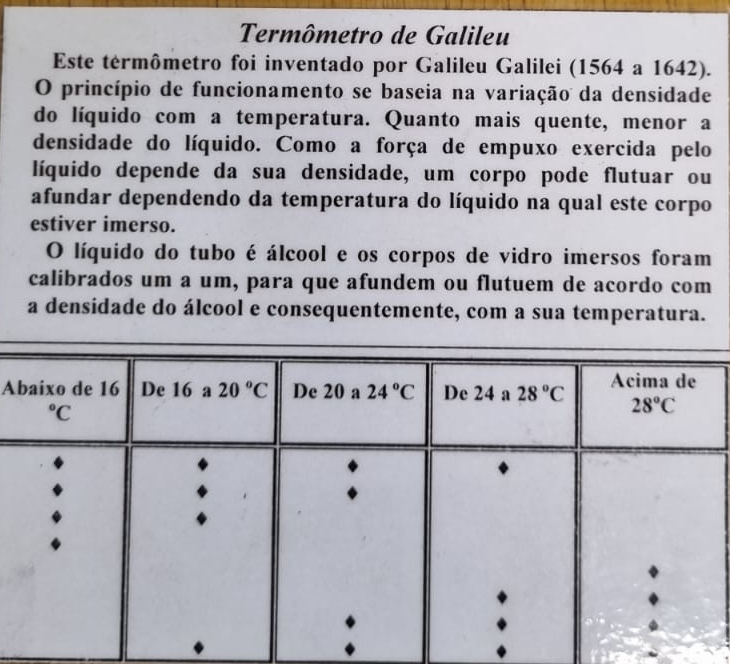
\includegraphics[width=.5\linewidth]{fig/temps}
    \caption{Temperaturas nominais e posições esperadas dos bonecos para cada uma}\label{temps}
\end{figure}

De toda forma, o princípio por trás deste experimento é a variação da densidade do líquido com a variação da temperatura. Ao aquecer, as moléculas que compõe o líquido têm maior energia cinética, aumentando, em média, a distância entre as moléculas do líquido. Desta forma, um objeto submerso no líquido está sujeito à força de empuxo deste, por sua vez, a força de empuxo varia com a densidade do líquido. Ao aumentar a temperatura a densidade do líquido diminui. Por consequência, aumento na temperatura resulta em diminuição da força de empuxo. Como os bonecos também estão sujeitos à força gravitacional, atuando sobre eles sem variação, na mesma direção e em sentido oposto ao da força de empuxo, ao diminuir a força de empuxo a força resultante se torna não nula e faz com que o boneco afunde um pouco mais. O contrário acontece ao resfriar o líquido. 

O termômetro de Galileu é um precursor engenhoso dos termômetros de mercúrio. Uma vantagem interessante deste em relação ao anterior é que não depende do uso de metais pesados. Porém, a resolução do termômetro de galileu depende de ajustar densidades muito próximas entre os objetos de medida, os bonecos no nosso caso. Além disso, o alcance de temperaturas mensuráveis com um termômetro de Galileu é limitado, não pode medir temperaturas próximas à temperatura de ebulição ou fusão do líquido utilizado.
